\documentclass[11pt]{article}
% anderweitig wiederverwendbare Makros fuer Diss
\usepackage{amsfonts}

% allgemeine mathematische Notation
\newcommand{\ceil}[1]{\left\lceil #1\right\rceil}
\newcommand{\floor}[1]{\left\lfloor #1\right\rfloor}
\newcommand{\abs}[1]{\left| #1\right|}
\newcommand{\seq}[1]{\langle #1\rangle}
\newcommand{\norm}[1]{\left\|#1\right\|}
\newcommand{\enorm}[1]{\norm{#1}_{2}}
\newcommand{\sumnorm}[1]{\norm{#1}_{1}}
\newcommand{\maxnorm}[1]{\norm{#1}_{\infty}}
\newcommand{\xor}{\oplus}
\newcommand{\set}[1]{\left\{ #1\right\}}
\newcommand{\gilt}{:}
\newcommand{\sodass}{\,:\,}
\newcommand{\setGilt}[2]{\left\{ #1\sodass #2\right\}}
\newcommand{\Def}{:=}
\newcommand{\zvektor}[2]{\left(#1,#2\right)}
\newcommand{\vektor}[2]{\left(\begin{smallmatrix}#1\\#2\end{smallmatrix}\right)}
\newcommand{\condition}[1]{\left[#1\right]}
\newcommand{\binomial}[2]{\binom{#1}{#2}}
\newcommand{\even}{\mathrm{even}}
\newcommand{\odd}{\mathrm{odd}}
\newcommand{\mymod}{\,\bmod\,}
\newcommand{\divides}{|}

\newcommand{\blank}{\Box}
\newcommand{\cross}[2]{\langle #1,#2 \rangle}
\newcommand{\defeq}{\mathrel{:=}}
\newcommand{\hash}{\sym{@}}
\newcommand{\hD}[1][D]{^{(#1)}}
\newcommand{\hed}[1][D]{^{1/#1}}
\newcommand{\Lpal}{L_{\mathrm{pal}}}
\newcommand{\Lparity}{L_{\mathrm{parity}}}
\newcommand{\Lvv}{L_{\mathrm{vv}}}
\newcommand{\pD}[1][D]{^{[#1]}}
\newcommand{\pos}[1]{\mathbf{#1}}
\newcommand{\qs}{\mathord{\Box}}
\newcommand{\mSet}[2]{\left\{#1 \mid #2\right\}}
\newcommand{\s}{\mathord{-}}
\newcommand{\CAce}{\hbox{\mdseries\scshape CAce}}
\newcommand{\sCAce}{\s\CAce}
\newcommand{\CAcs}{\hbox{\mdseries\scshape CAcs}}
\newcommand{\sCAcs}{\s\CAcs}
\newcommand{\CAww}{\hbox{\mdseries\scshape CAww}}
\newcommand{\sCAww}{\s\CAww}
\newcommand{\sC}{\s\hbox{\scshape Chng}}
\newcommand{\sD}{\s\hbox{\scshape Diam}}
\newcommand{\sT}{\s\hbox{\scshape Time}}
\newcommand{\CA}{\hbox{\mdseries\scshape CA}}
\newcommand{\sCA}{\s\CA}
\newcommand{\ST}[1]{\langle #1\rangle}
\newcommand{\sym}[1]{\mathord{\hbox{\texttt{\upshape #1}}}}

% Typen
\newcommand{\nat}{\mathbb{N}}
\newcommand{\natnull}{\mathbb{N}_{0}}
%\newcommand{\natless}[1]{\mathbb{N}_{<#1}}
\newcommand{\natless}[1]{\mathbb{N}_{#1}}
\newcommand{\nplus}{\mathbb{N}_+}
\newcommand{\real}{\mathbb{R}}
\newcommand{\rplus}{\mathbb{R}_+}
\newcommand{\rnneg}{\mathbb{R}_*}
\newcommand{\integer}{\mathbb{Z}}
% \newcommand{\intint}[2]{\set{#1,\ldots, #2}}
\newcommand{\intint}[2]{{#1}..{#2}}
\newcommand{\realrange}[2]{\left[#1, #2\right]}
\newcommand{\realrangeo}[2]{\left(#1, #2\right)}
\newcommand{\realrangelo}[2]{\left(#1, #2\right]}
\newcommand{\realrangero}[2]{\left[#1, #2\right)}
\newcommand{\unitrange}[2]{\realrange{0}{1}}
\newcommand{\bool}{\set{0,1}}
%\newcommand{\boolean}{\mathbb{B}}
%\newcommand{\mapping}[2]{#1\rightarrow #2}
\newcommand{\mapping}[2]{{#2}^{#1}}
\newcommand{\powerset}[1]{{\cal P}\left(#1\right)}
\newcommand{\NP}{\mathbf{NP}}
\newcommand{\Bild}{\mathbf{Bild}\:}

% Typannotation
\newcommand{\withtype}[1]{\in#1}

% Wahrscheinlichkeitsrechnung
\newcommand{\prob}[1]{{\mathbf{P}}\left[#1\right]}
\newcommand{\condprob}[2]{{\mathbf{P}}\left[#1\;|\;#2\right]}
\newcommand{\condexpect}[2]{{\mathbf{E}}\left[#1\;|\;#2\right]}
\newcommand{\expect}{{\mathbf{E}}}
\newcommand{\var}{{\mathbf{Var}}}
\newcommand{\quant}[2]{\tilde{#1}_{#2}}

% asymptotische Notation
\newcommand{\whpO}[1]{\tilde{\mathrm{O}}\left( #1\right)}
\newcommand{\Oschlange}{$\tilde{\mathrm{O}}$}
\newcommand{\Ohh}[1]{\mathcal{O}\!\left( #1\right)}
\newcommand{\Oh}[1]{\mathcal{O}\!\left( #1\right)}
\newcommand{\oh}[1]{\mathrm{o}\!\left( #1\right)}
\newcommand{\Th}[1]{\Theta\!\left( #1\right)}
\newcommand{\Thsmall}[1]{\Theta( #1)}
\newcommand{\Om}[1]{\Omega\!\left( #1\right)}
\newcommand{\om}[1]{\omega\!\left( #1\right)}
\newcommand{\Oleq}{\preceq}

% local reference
\newcommand{\lref}[1]{\ref{\labelprefix:#1}}
\newcommand{\llabel}[1]{\label{\labelprefix:#1}}
\newcommand{\labelprefix}{} % later redefined using renewcommand

% Diskussion
\newcommand{\discussionsize}{\small}
\newenvironment{discussion}{\par\discussionsize}{\par}

% open issues
%\marginparwidth5cm
\marginparpush2mm
%\newcommand{\frage}[1]{\makebox[0cm]{$\bigotimes$}\marginpar{\tiny #1}}
%\newcommand{\frage}[1]{{\sf[ #1]}\marginpar{?}}
\newcommand{\frage}[1]{}

\newcommand{\mysubsubsection}[1]{\vspace{2mm}\noindent{\bf #1 }}

% punkt am ende von display math
\newcommand{\punkt}{\enspace .}

% Pseudocode Unterst\"utzung
\newenvironment{code}{\noindent%\sf%
\begin{tabbing}%
\hspace{2em}\=\hspace{2em}\=\hspace{2em}\=\hspace{2em}\=\hspace{2em}\=%
\hspace{2em}\=\hspace{2em}\=\hspace{2em}\=\hspace{2em}\=\hspace{2em}\=%
\kill}{\end{tabbing}}

% 1=pos, 2=llable, 3=caption
\newcommand{\labelcommand}{}
\newcommand{\captiontext}{}
\newsavebox{\codeparam}
\newcounter{lineNumber}
\newenvironment{disscodepos}[3]{%
\renewcommand{\labelcommand}{#2}%
\renewcommand{\captiontext}{#3}%
\sbox{\codeparam}{\parbox{\textwidth}{#3}}%
\begin{figure}[#1]\begin{center}\begin{code}\setcounter{lineNumber}{1}}{%
\end{code}\end{center}\caption{\llabel{\labelcommand}\captiontext}\end{figure}}

\newenvironment{disscode}[2]{\begin{disscodepos}{htb}{#1}{#2}}%
{\end{disscodepos}}

% code in text 
%\newcommand{\codel}[1]{{\sf #1}}
%\newcommand{\codem}[1]{\mathsf{#1}}
\newcommand{\codel}[1]{\mbox{\rm "`#1"'}}
\newcommand{\codem}[1]{\mathrm{#1}}

\newcommand{\id}{\tt}
\newcommand{\Function} {{\bf Function\ }}
\newcommand{\Procedure}{{\bf Procedure\ }}
\newcommand{\Process}{{\bf process\ }}
\newcommand{\While}    {{\bf while\ }}
\newcommand{\Repeat}   {{\bf repeat\ }}
\newcommand{\Until}    {{\bf until\ }}
\newcommand{\Loop}     {{\bf loop\ }}
\newcommand{\Exit}     {{\bf exit\ }}
\newcommand{\Goto}     {{\bf goto\ }}
\newcommand{\Do}       {{\bf do\ }}
\newcommand{\Od}       {{\bf od\ }}
\newcommand{\Dopar}       {{\bf dopar\ }}
\newcommand{\For}      {{\bf for\ }}
\newcommand{\Step}      {{\bf step\ }}
\newcommand{\Foreach}      {{\bf foreach\ }}
\newcommand{\Rof}      {{\bf rof\ }}
\newcommand{\Forall}      {{\bf forall\ }}
\newcommand{\To}       {{\bf to\ }}
\newcommand{\If}       {{\bf if\ }}
\newcommand{\Is}       {:=}
\newcommand{\Endif}    {{\bf endif\ }}
\newcommand{\Fi}       {{\bf fi\ }}
\newcommand{\Then}     {{\bf then\ }}
\newcommand{\Else}     {{\bf else\ }}
\newcommand{\Elsif}    {{\bf elsif\ }}
\newcommand{\Return}   {{\bf return\ }}
\newcommand{\Set}      {{\bf set\ }}
\newcommand{\Boolean}  {{\bf boolean\ }}
\newcommand{\Integer}  {$\integer$}
\newcommand{\True}     {{\bf true\ }}
\newcommand{\False}    {{\bf false\ }}
\newcommand{\Bitand}   {{\bf bitand\ }}
\newcommand{\Var}      {{\bf var\ }}
\newcommand{\Xor}       {{\bf\ xor\ }}
\newcommand{\Not}       {{\bf\ not\ }}
\newcommand{\Or}       {{\bf\ or\ }}
\newcommand{\Div}       {{\bf\ div\ }}
\newcommand{\Mod}       {{\bf\ mod\ }}
\newcommand{\End}       {{\bf end\ }}
\newcommand{\Endfor}       {{\bf endfor\ }}
\newcommand{\Rem}[1]   {{\bf (*~}{\rm#1}{\bf ~*)}}
% rechtsbuendiger Kommentar
%\newcommand{\RRem}[1]   {\`{$\mathbf{(*}$~ }{\rm#1}{~$\mathbf{*)}$}}
\newcommand{\RRem}[1]   {\`{\bf --\hspace{0.5mm}--~}{\rm#1}}
\newcommand{\RRemNL}[1]   {\`{\bf (*~ }{\rm#1}{\bf ~*)}%
{\tiny\arabic{lineNumber}}\stepcounter{lineNumber}}

\newcommand{\At}[1]{\left\langle#1\right\rangle}
\newcommand{\NL}{\`{\tiny\arabic{lineNumber}}\stepcounter{lineNumber}}

% Parallelverarbeitungspseudocode
\newcommand{\iProc}{i_\mathrm{PE}}

% Parameter 1=pos, 2=xsize, 3=filename, 4=llabel, 4=caption
\newcommand{\dissepslong}[5]{\begin{figure}[#1]\begin{center}%
\epsfxsize#2\leavevmode\epsfbox{#3.eps}%
\end{center}\caption{\llabel{#4}#5}\end{figure}}

\newcommand{\dissepspos}[4]{\dissepslong{#1}{#2}{\labelprefix/#3}{#3}{#4}}
\newcommand{\disseps}[3]{\dissepspos{htb}{#1}{#2}{#3}}

% Beweise
\newdimen\endofsize\endofsize=0.5em
\def\endofbeweis{~\quad\hglue\hsize minus\hsize
                 \hbox{\vrule height \endofsize width
\endofsize}\par}
% gibt es in amsmath schon
\newenvironment{myproof}{\begin{proof}}{\endofbeweis\end{proof}}
% \newcommand{\platsch}{\hglue\hsize minus\hsize}

\newif\ifFull
\Fullfalse

\usepackage[utf8]{inputenc}
\usepackage{algorithmic}
\usepackage{tabularx}
\usepackage{algorithm}
\usepackage{theorem}
\usepackage{amsmath}
\usepackage{amssymb}
\usepackage{color}
\usepackage{fullpage}     
\usepackage{latexsym}
\usepackage{makeidx}
\usepackage{multicol}
\usepackage{numprint}
\usepackage{t1enc}
\usepackage{times}
\usepackage{graphicx}
\usepackage{url}
\usepackage[left=2cm,top=1.5cm,right=2cm]{geometry}
\npdecimalsign{.} % we want . not , in numbers

\definecolor{mygrey}{gray}{0.75}
\newcommand{\ie}{i.e.\ }
\newcommand{\etal}{et~al.\ }
\newcommand{\eg}{e.g.\ }
\newcommand{\Id}[1]{\ensuremath{\text{{\sf #1}}}}

\def\MdR{\ensuremath{\mathbb{R}}}
\def\MdN{\ensuremath{\mathbb{N}}}
\newcommand{\mytodo}[1]{{\color{blue}#1}}
\newcommand{\sout}[1]{{\color{mygrey}#1}}

\newcommand{\mytitle}{ {\color{red}KaMIS} v1.0 -- {\color{red}Ka}rlsruhe {\color{red}M}aximum {\color{red}I}ndependent {\color{red}S}ets \\ User Guide}
\begin{document}
\title{\mytitle}
\author{Sebastian Lamm, Peter Sanders, Christian Schulz, Darren Strash and Renato F. Werneck\\ 
	\textit{Karlsruhe Institute of Technology (KIT)},
	\textit{Karlsruhe, Germany} \\
    \textit{\url{lamm@ira.uka.de}, \{\url{sanders}, \url{christian.schulz}, \url{strash}\}\url{@kit.edu}} \\
	\textit{San Francisco, USA} \\
    \textit{\url{rwerneck@acm.org}}}
\date{}

\maketitle
\begin{abstract}
This paper serves as a user guide to the framework KaMIS (Karlsruhe Maximum Independent Sets). 
The framework computes high quality independent sets in huge sparse graphs.
We give a rough overview of the techniques used within the framework and describe the user interface as well as the file formats used. 
\end{abstract}

\tableofcontents
\thispagestyle{empty}

\vfill
\pagebreak
\section{Introduction}
The maximum independent set problem is an NP-hard problem that has attracted much attention in the combinatorial optimization community, due to its difficulty and its importance in many fields. Given a graph $G=(V,E)$, the goal of the maximum independent set problem is to compute a maximum cardinality set of vertices $\mathcal{I}\subseteq V$, such that no vertices in $\mathcal{I}$ are adjacent to one another. Such a set is called a \emph{maximum independent set} (MIS). The maximum independent set problem has applications spanning many disciplines, including classification theory, information retrieval, and computer vision~\cite{feo1994greedy}.
\ifFull
As a concrete example, independent sets are vital in labeling strategies for maps~\cite{gemsa2014dynamiclabel}. Here, the objective is to maximize the number of visible non-overlapping labels on a map. 
In this example, the maximum independent set problem is solved in the label conflict graph, in which any two conflicting/overlapping labels are connected by an edge.
\else
Independent sets are also used in efficient strategies for labeling maps~\cite{gemsa2014dynamiclabel}, computing shortest paths on road networks~\cite{kieritz-contraction-2010}, (via the complementary minimum vertex cover problem) computing mesh edge traversal ordering for rendering~\cite{sander-mesh-2008}, and (via the complementary maximum clique problem) have applications in biology~\cite{gardiner-docking-2000}, sociology~\cite{harary-clique-1957}, and e-commerce~\cite{zaki-ecommerce-97}.
\fi

It is easy to see that the complement of an independent set $\mathcal{I}$ is a vertex cover $V \backslash \mathcal{I}$ and an independent set in $G$ is a clique in the complement graph $\overline{G}$. 
Since all of these problems are NP-hard~\cite{DBLP:books/fm/GareyJ79}, heuristic
algorithms are used in practice to efficiently compute solutions of high quality on \emph{large} graphs~\cite{AndradeRW12,grosso2008simple}. However, small graphs with hundreds to thousands of vertices may often be solved in practice with traditional branch-and-bound methods~\cite{segundo-recoloring,segundo-bitboard-2011,tomita-recoloring}, and medium-sized instances can be solved exactly in practice using reduction rules to kernelize the graph. Recently, Akiba and Iwata~\cite{akiba-2015} used advanced reduction rules with a measure and conquer approach to solve the minimum vertex cover problem for medium-scale sparse graphs exactly in practice. Thus, their algorithm also finds the maximum independent set for these instances.  
However, none of these exact algorithms can handle huge sparse graphs. Furthermore, our experiments suggest that the quality of existing heuristic-based solutions tends to degrade at scale for inputs such as Web graphs and road networks. Therefore, we need new techniques to find high-quality independent sets in these graphs.

With KaMIS we provide a framework for computing high quality independent sets in huge sparse graphs.
So far our framework contains the ReduMIS algorithm which is an advanced evolutionary algorithm based on graph partitioning and incorporates kernelization techniques to compute large independent sets. 
Our algorithm uses reduction techniques and recursively chooses vertices that are likely to be in a large independent set (using an evolutionary approach), to then further kernelize the graph. 
This opens up the reduction space -- which not only speeds up the computation of large independent sets drastically, but also enables us to compute high-quality independent sets on massive instances. 

\vfill
\pagebreak
\,
\pagebreak

\section{Algorithmic components within KaMIS}
We now give a rough overview over the algorithmic components implemented in our framework. For details on the individual components, we refer the interested reader to the corresponding papers. 

\paragraph{ARW.}
There is a wide range of heuristics and local search algorithms for the maximum clique problem (see for example \cite{battiti2001reactive,hansen2004variable,grosso2004combining,katayama2005effective,pullan2006dynamic,grosso2008simple}). 
They typically maintain a single solution and try to improve it by performing node deletions, insertions, and swaps, as well as \emph{plateau} search. 
For the independent set problem, Andrade \etal\cite{AndradeRW12} extended the notion of swaps to $(j,k)$-swaps, which remove $j$ nodes from the current solution and insert $k$ nodes. 
One \emph{iteration} of the ARW algorithm consists of a perturbation and a local search step.
The ARW \emph{local search} algorithm uses simple $2$-improvements or $(1,2)$-swaps to gradually improve a single current solution.  
The simple version of the local search iterates over all nodes of the graph and looks for a $(1,2)$-swap. 
By using a data structure that allows insertion and removal operations on nodes in time proportional to their degree, this procedure can find a valid $(1,2)$-swap in $\mathcal{O}(m)$ time, if it exists.
An even faster incremental version of the algorithm (which we use here) maintains a list of \emph{candidates}, which are nodes that may be involved in $(1,2)$-swaps. 
It ensures a node is not examined twice unless there is some change in its neighborhood.

\paragraph{EvoMIS.}
EvoMIS is a very natural evolutionary algorithm proposed by Lamm~\etal\cite{lammSEA2015}. 
It uses combination operations that are based on graph partitioning and ARW local search.
They employ the partitioning framework KaHIP~\cite{kabapeE} to derive operations that make it possible to quickly exchange whole blocks of given independent sets. 

The basic idea of the combine operations is to use a partition of the graph to exchange whole blocks of solution nodes and use local search afterwards to turn the solution into a maximal one.
We explain one of the combine operations based on 2-way node separators in more detail.
In its simplest form, the operator starts by computing a 2-way node separator $V=V_1 \cup V_2 \cup S$ of the input graph. 
The separator $S$ is then used as a crossover point for the operation.
The operator generates two children, $O_1=(V_1\cap \mathcal{I}_1) \cup (V_2\cap\mathcal{I}_2)$ and $O_2=(V_1\cap \mathcal{I}_2) \cup (V_2\cap\mathcal{I}_1)$.  
In other words, whole parts of independent sets are exchanged from the blocks $V_1$ and $V_2$ of the node separator. 
Note that the exchange can be implemented in time linear in the number of nodes.
Recall that a node separator ensures that there are no edges between $V_1$ and $V_2$.
Hence, the computed children are independent sets, but may not be maximal since separator nodes have been ignored and potentially some of them can be added to the solution.
Therefore, the child is made maximal by using a greedy algorithm. 
The operator finishes with one iteration of the ARW algorithm to ensure that a local optimum is reached and to add diversification.

\paragraph{Reduction Techniques.}
Our algorithm uses exact and inexact reduction techniques to shrink the search space.
Each reduction allows us to choose vertices that are in some MIS by following simple rules. If an MIS is found on the kernel graph $\mathcal{K}$, then each reduction may be undone, producing an MIS in the original graph. Refer to Akiba and Iwata~\cite{akiba-2015} for a more thorough discussion, including implementation details. 
With these facts in mind, we apply the evolutionary algorithm on the  kernelized graph instead of on the input graph, thus boosting its performance.
We use intermediate solutions of the evolutionary algorithm to select good solution candidates (independent set vertices), remove them and their incident neighbors from the graph, and finally repeat the whole process. For more details on the algorithm, we refer the reader to \cite{alx2016IS}.
\\

\vfill
\pagebreak
\,
\pagebreak
\section{Graph Format}
\label{ss:graphformat}
\subsection{Input File Format}
The graph format used by our partitioning programs is the same as used by Metis \cite{karypis1998fast}, Chaco \cite{chaco} and the graph format that has been used during the 10th DIMACS Implementation Challenge on Graph Clustering and Partitioning. 
The input graph has to be undirected, without self-loops and without parallel edges.

To give a description of the graph format, we follow the description of the Metis 4.0 user guide very closely. A graph $G=(V,E)$ with $n$ vertices and $m$ edges is stored in a plain text file that contains $n+1$ lines (excluding comment lines). The first line contains information about the size and the type of the graph, while the remaining $n$ lines contain information for each vertex of $G$. Any line that starts with \% is a comment line and is skipped.

The first line in the file contains two integers $n$ $m$. The two integers are the number of vertices $n$ and the number of undirected edges of the graph, respectively. Note that in determining the number of edges $m$, an edge between any pair of vertices $v$ and $u$ is counted \emph{only once} and not twice, \ie we do not count the edge $(v,u)$ from $(u,v)$ separately. 
The remaining $n$ lines of the file store information about the actual structure of the graph. In particular, the $i$th line (again excluding comment lines) contains information about the $i$th vertex.
Each line has the following structure:
\begin{center}
       $v_1\, v_2\,  \ldots v_k$ 
\end{center}
where $v_1, \ldots, v_k$ are the vertices adjacent to the vertex described by the line. 
The adjacent vertices must be \emph{sorted} by increasing order.
Note that the vertices are numbered starting from 1 (not from 0). 

\begin{figure}[b]
\centering
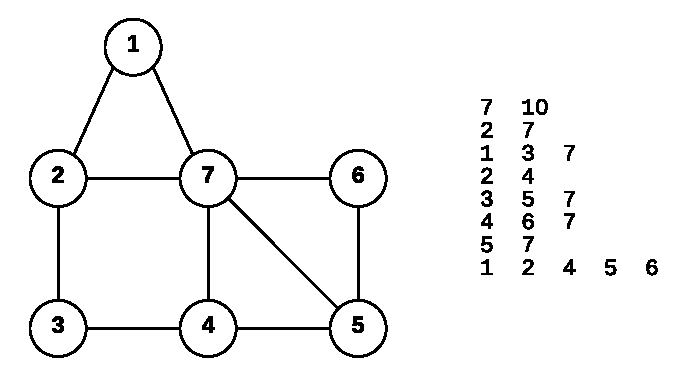
\includegraphics[scale=0.7]{input_format.pdf}
\caption{An example graph and its representation in the graph format.}
\label{fig:inputformat}
\end{figure}

\subsection{Output File Formats}
The output format is basically a text file that represents the independent set. 
This file contains $n$ lines. 
Each line indicates if the corresponding vertex is part of the independent set ($1$) or not ($0$), i.e. line i indicates if vertex i (here the vertices are numbered from $0$ to $n-1$) is part of the independent set. 
\subsection{Troubleshooting}
KaMIS should not crash! If KaMIS crashes it is mostly due to the following reasons: the provided graph contains self-loops or parallel edges, the edges are not sorted, there exists a forward edge but the backward edge is missing, or the number of vertices or edges specified does not match the number of vertices or edges provided in the file.
To sort the edges of an unsorted graph please use the \texttt{sort\_metis.py} script in \texttt{misc/conversion}.
Please use the \emph{graphchecker} tool provided in our package to verify whether your graph has the right input format. 
If our graphchecker tool tells you that the graph that you provided has the correct format and KaMIS crashes anyway, please write us an email.

\vfill
\pagebreak
\section{User Interface}
KaMIS contains the program \texttt{redumis} to compute an independent set. 
To compile this program you need to have Argtable, g++, OpenMP and scons installed (we use argtable-2.10, g++-4.8.0 and scons-1.2). 
Once you have that you can execute \texttt{compile.sh} in the main folder of the release. 
When the process is finished the binaries can be found in the folder \texttt{deploy}. We now explain the parameters of each of the programs briefly.
\subsection{ReduMIS}
\paragraph*{Description:} This is the evolutionary algorithm based on graph partitioning and reduction techniques. 
\paragraph*{Usage:\\} 

\begin{tabular}{ll}
redumis &   [-{}-help] FILE [-{}-seed=<int>] [-{}-config=VARIANT]  [-{}-time\_limit=<double>] \\
& [-{}-output=<string>] [-{}-console\_log] [-{}-all\_reductions] [-{}-red\_thres=<int>]

\end{tabular}
                          
\subsection*{Options:\\}

\begin{tabularx}{\textwidth}{lX}
  FILE                          & Path to graph file.\\
  --help                        & Print help. \\
  --seed=<int>                  & Seed to use for the PRNG.\\
  --config=VARIANT              & Use a preconfiguration. (Default: standard) [standard|social|full\_standard|full\_social].\\
                                & Standard/social use different graph partitioning modes. \\ 
                                & "full" configurations use more time consuming parameters.\\
  --time\_limit=<double>        & Time limit. (Default: 1000s)\\
  --output=<string>             & Path to output file.\\
  --console\_log                & Print verbose output to the console.\\
  --disable\_checks             & Disable sortedness check during I/O.\\
  --red\_thres=<int>            & Number of unsuccessful iterations of EA before reduction (Default: 350).\\
\end{tabularx}


\subsection{Graph Format Checker}
\paragraph*{Description:} This program checks if the graph specified in a given file is valid. 
\paragraph*{Usage:\\} 
\begin{tabular}{ll}
graphchecker & file
\end{tabular}
\subsection*{Options:\\} 
\begin{tabularx}{\textwidth}{lX}
  FILE                       & Path to the graph file. \\
\end{tabularx}

\vfill
\pagebreak
\vfill
\pagebreak
\bibliographystyle{plain}
\begin{thebibliography}{10}

\bibitem{akiba-2015}
T.~Akiba and Y.~Iwata.
\newblock {Branch-and-reduce Exponential/FPT Algorithms in Practice: A Case
  Study of Vertex Cover}.
\newblock In {\em Proceedings of the Meeting on Algorithm Engineering \&
  Expermiments}, ALENEX '15, pages 70--81, Philadelphia, PA, USA, 2015. Society
  for Industrial and Applied Mathematics.

\bibitem{AndradeRW12}
D.~V. Andrade, M.~G.~C. Resende, and R.~F. Werneck.
\newblock {Fast Local Search for the Maximum Independent Set Problem}.
\newblock {\em Journal of Heuristics}, 18(4):525--547, 2012.

\bibitem{battiti2001reactive}
R.~Battiti and M.~Protasi.
\newblock {Reactive Local Search for the Maximum Clique Problem}.
\newblock {\em Algorithmica}, 29(4):610--637, 2001.

\bibitem{feo1994greedy}
T.~A. Feo, M.~G.~C. Resende, and S.~H. Smith.
\newblock {A Greedy Randomized Adaptive Search Procedure for Maximum
  Independent Set}.
\newblock {\em Operations Research}, 42(5):860--878, 1994.

\bibitem{gardiner-docking-2000}
Eleanor~J. Gardiner, , Peter Willett, and Peter~J. Artymiuk.
\newblock Graph-theoretic techniques for macromolecular docking.
\newblock {\em Journal of Chemical Information and Computer Science},
  40(2):273--279, 2000.

\bibitem{DBLP:books/fm/GareyJ79}
M.~R. Garey and David~S. Johnson.
\newblock {\em {Computers and Intractability: {A} Guide to the Theory of
  NP-Completeness}}.
\newblock W. H. Freeman, 1979.

\bibitem{gemsa2014dynamiclabel}
A.~Gemsa, M.~Nöllenburg, and I.~Rutter.
\newblock Evaluation of labeling strategies for rotating maps.
\newblock In {\em Experimental Algorithms}, volume 8504 of {\em LNCS}, pages
  235--246. Springer, 2014.

\bibitem{grosso2004combining}
A.~Grosso, M.~Locatelli, and F.~Della~C.
\newblock {Combining Swaps and Node Weights in an Adaptive Greedy Approach for
  the Maximum Clique Problem}.
\newblock {\em Journal of Heuristics}, 10(2):135--152, 2004.

\bibitem{grosso2008simple}
A.~Grosso, M.~Locatelli, and W.~Pullan.
\newblock {Simple Ingredients Leading to Very Efficient Heuristics for the
  Maximum Clique Problem}.
\newblock {\em Journal of Heuristics}, 14(6):587--612, 2008.

\bibitem{hansen2004variable}
P.~Hansen, N.~Mladenovi{\'c}, and D.~Uro{\v{s}}evi{\'c}.
\newblock {Variable Neighborhood Search for the Maximum Clique}.
\newblock {\em Discrete Applied Mathematics}, 145(1):117--125, 2004.

\bibitem{harary-clique-1957}
F.~Harary and I.~C. Ross.
\newblock {A Procedure for Clique Detection Using the Group Matrix}.
\newblock {\em Sociometry}, 20(3):pp. 205--215, 1957.

\bibitem{chaco}
B.~Hendrickson.
\newblock {Chaco: Software for Partitioning Graphs}.
\newblock {\url{http://www.cs.sandia.gov/~bahendr/chaco.html}}.

\bibitem{iwata-2014}
Y.~Iwata, K.~Oka, and Y.~Yoshida.
\newblock {Linear-time FPT Algorithms via Network Flow}.
\newblock In {\em Proceedings of 25th ACM-SIAM Symposium on Discrete
  Algorithms}, SODA '14, pages 1749--1761. SIAM, 2014.

\bibitem{karypis1998fast}
G.~Karypis and V.~Kumar.
\newblock {A Fast and High Quality Multilevel Scheme for Partitioning Irregular
  Graphs}.
\newblock {\em SIAM Journal on Scientific Computing}, 20(1):359--392, 1998.

\bibitem{katayama2005effective}
K.~Katayama, A.~Hamamoto, and H.~Narihisa.
\newblock {An Effective Local Search for the Maximum Clique Problem}.
\newblock {\em Information Processing Letters}, 95(5):503--511, 2005.

\bibitem{kieritz-contraction-2010}
T.~Kieritz, D.~Luxen, P.~Sanders, and C.~Vetter.
\newblock Distributed time-dependent contraction hierarchies.
\newblock In Paola Festa, editor, {\em Experimental Algorithms}, volume 6049 of
  {\em LNCS}, pages 83--93. Springer Berlin Heidelberg, 2010.

\bibitem{lammSEA2015}
S.~Lamm, P.~Sanders, and C.~Schulz.
\newblock {Graph Partitioning for Independent Sets}.
\newblock In {\em Proceedings of the 14th International Symposium on
  Experimental Algorithms (SEA'15)}, volume 8504, pages 68--81. Springer, 2015.

\bibitem{pcomplexnetworksviacluster}
H.~Meyerhenke, P.~Sanders, and C.~Schulz.
\newblock {Partitioning Complex Networks via Size-constrained Clustering}.
\newblock In {\em 13th Int. Symp. on Exp. Algorithms}, LNCS. Springer, 2014.

\bibitem{nemhauser-1975}
G.L. Nemhauser and Jr. Trotter, L.E.
\newblock Vertex packings: Structural properties and algorithms.
\newblock {\em Mathematical Programming}, 8(1):232--248, 1975.

\bibitem{pullan2006dynamic}
W.~J. Pullan and H.~H. Hoos.
\newblock {Dynamic Local Search for the Maximum Clique Problem}.
\newblock {\em Journal of Artifical Intelligence Research(JAIR)}, 25:159--185,
  2006.

\bibitem{segundo-recoloring}
P.~San~Segundo, F.~Matia, D.~Rodriguez-Losada, and M.~Hernando.
\newblock An improved bit parallel exact maximum clique algorithm.
\newblock {\em Optimization Letters}, 7(3):467--479, 2013.

\bibitem{segundo-bitboard-2011}
P.~San~Segundo, D.~Rodríguez-Losada, and Agustín J.
\newblock An exact bit-parallel algorithm for the maximum clique problem.
\newblock {\em Computers \& Operations Research}, 38(2):571--581, 2011.

\bibitem{sander-mesh-2008}
P.~V. Sander, D.~Nehab, E.~Chlamtac, and H.~Hoppe.
\newblock Efficient traversal of mesh edges using adjacency primitives.
\newblock {\em ACM Trans. Graph.}, 27(5):144:1--144:9, December 2008.

\bibitem{kaHIPHomePage}
P.~Sanders and C.~Schulz.
\newblock {KaHIP -- Karlsruhe High Qualtity Partitioning Homepage}.
\newblock {\url{http://algo2.iti.kit.edu/documents/kahip/index.html}}.

\bibitem{kabapeE}
P.~Sanders and C.~Schulz.
\newblock {Think Locally, Act Globally: Highly Balanced Graph Partitioning}.
\newblock In {\em Proceedings of the 12th International Symposium on
  Experimental Algorithms (SEA'13)}, LNCS. Springer, 2013.

\bibitem{tomita-recoloring}
E.~Tomita, Y.~Sutani, T.~Higashi, S.~Takahashi, and M.~Wakatsuki.
\newblock A simple and faster branch-and-bound algorithm for finding a maximum
  clique.
\newblock In Md.~Saidur Rahman and Satoshi Fujita, editors, {\em WALCOM:
  Algorithms and Computation}, volume 5942 of {\em LNCS}, pages 191--203.
  Springer Berlin Heidelberg, 2010.

\bibitem{Xiao201392}
M.~Xiao and H.~Nagamochi.
\newblock Confining sets and avoiding bottleneck cases: A simple maximum
  independent set algorithm in degree-3 graphs.
\newblock {\em Theoretical Computer Science}, 469:92 -- 104, 2013.

\bibitem{zaki-ecommerce-97}
M.~J. Zaki, S.~Parthasarathy, M.~Ogihara, and W.~Li.
\newblock {New Algorithms for Fast Discovery of Association Rules}.
\newblock In {\em 3rd International Conference on Knowledge Discovery and Data
  Mining}, pages 283--286. AAAI Press, 1997.

\bibitem{alx2016IS}
S. Lamm, P. Sanders, C. Schulz, D. Strash and R. F. Werneck
\newblock {Finding Near-Optimal Independent Sets at Scale}.
\newblock In {\em Proceedings of the 16th Workshop on Algorithm Engineering and Experimentation (ALENEX'16)}. 2016.

\end{thebibliography}

\end{document}

